\section{Operativ systemet}

\begin{figure}[h!]
	\centering
	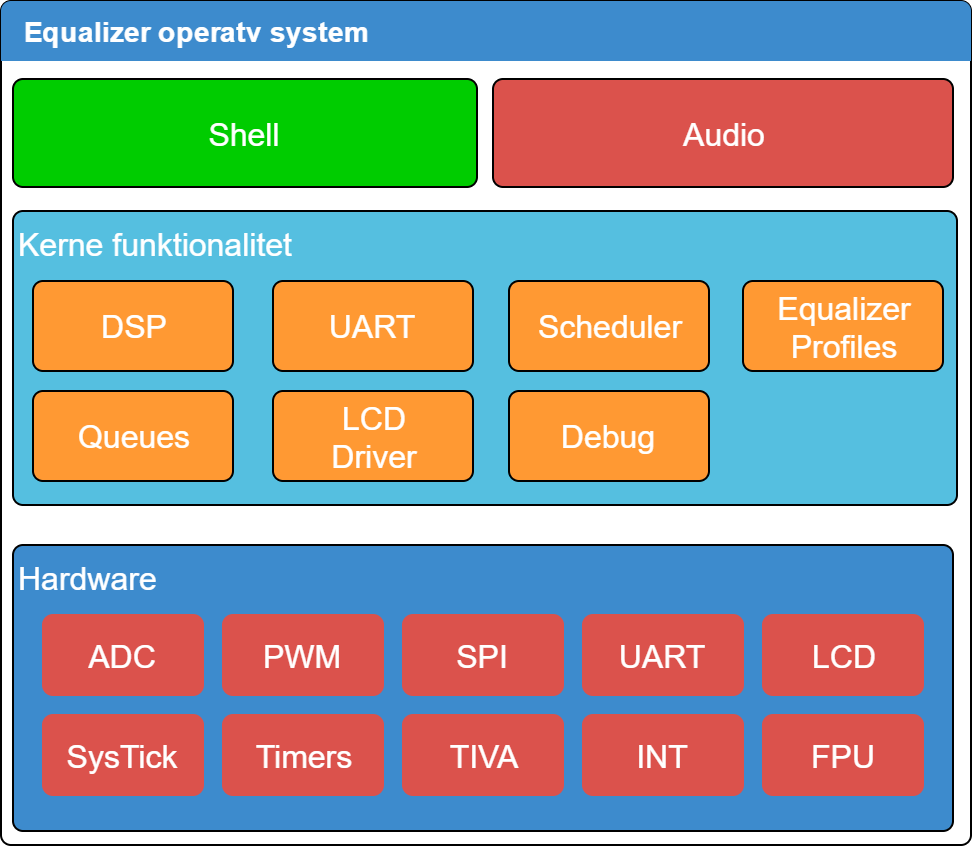
\includegraphics[width=.5\textwidth]{billeder/eq_os.png}
	\caption{Arkitektur af equalizerens operativ system.}
	\label{fig:eq_os}
\end{figure}

Figur viser et lagdelt OS.

Lavest lag er hardware konfiguration og dele der bliver brugt af equalizer.

Gennemgang af hver hardware dels opsætning samt det begrundede beslutninger er taget ved valget.

Kerne funktionalitets lag indeholder funktionalitet til at servicere systemet.
Herunder - UART til seriel kommunikation (SHELL), DSP funktionalitet til at lave beregninger for filtre, Scheduler som søger for at køre hele OS, Equalizer modul til at håndtere equalizer base funktionalitet samt håndtering af profiler. Service moduler som LCD driver, queues og debug funktionalitet.

User level funktionalitet : SHELL og Audio

Dette er top level funktionalitet : SHELL er brugeres tilgang til systemet, og audio er "lydens" tilgang til systemet.


\FloatBlock